\documentclass{article}\usepackage[]{graphicx}\usepackage[]{xcolor}
% maxwidth is the original width if it is less than linewidth
% otherwise use linewidth (to make sure the graphics do not exceed the margin)
\makeatletter
\def\maxwidth{ %
  \ifdim\Gin@nat@width>\linewidth
    \linewidth
  \else
    \Gin@nat@width
  \fi
}
\makeatother

\definecolor{fgcolor}{rgb}{0.345, 0.345, 0.345}
\newcommand{\hlnum}[1]{\textcolor[rgb]{0.686,0.059,0.569}{#1}}%
\newcommand{\hlsng}[1]{\textcolor[rgb]{0.192,0.494,0.8}{#1}}%
\newcommand{\hlcom}[1]{\textcolor[rgb]{0.678,0.584,0.686}{\textit{#1}}}%
\newcommand{\hlopt}[1]{\textcolor[rgb]{0,0,0}{#1}}%
\newcommand{\hldef}[1]{\textcolor[rgb]{0.345,0.345,0.345}{#1}}%
\newcommand{\hlkwa}[1]{\textcolor[rgb]{0.161,0.373,0.58}{\textbf{#1}}}%
\newcommand{\hlkwb}[1]{\textcolor[rgb]{0.69,0.353,0.396}{#1}}%
\newcommand{\hlkwc}[1]{\textcolor[rgb]{0.333,0.667,0.333}{#1}}%
\newcommand{\hlkwd}[1]{\textcolor[rgb]{0.737,0.353,0.396}{\textbf{#1}}}%
\let\hlipl\hlkwb

\usepackage{framed}
\makeatletter
\newenvironment{kframe}{%
 \def\at@end@of@kframe{}%
 \ifinner\ifhmode%
  \def\at@end@of@kframe{\end{minipage}}%
  \begin{minipage}{\columnwidth}%
 \fi\fi%
 \def\FrameCommand##1{\hskip\@totalleftmargin \hskip-\fboxsep
 \colorbox{shadecolor}{##1}\hskip-\fboxsep
     % There is no \\@totalrightmargin, so:
     \hskip-\linewidth \hskip-\@totalleftmargin \hskip\columnwidth}%
 \MakeFramed {\advance\hsize-\width
   \@totalleftmargin\z@ \linewidth\hsize
   \@setminipage}}%
 {\par\unskip\endMakeFramed%
 \at@end@of@kframe}
\makeatother

\definecolor{shadecolor}{rgb}{.97, .97, .97}
\definecolor{messagecolor}{rgb}{0, 0, 0}
\definecolor{warningcolor}{rgb}{1, 0, 1}
\definecolor{errorcolor}{rgb}{1, 0, 0}
\newenvironment{knitrout}{}{} % an empty environment to be redefined in TeX

\usepackage{alltt}
\usepackage[margin=1.0in]{geometry} % To set margins
\usepackage{amsmath}  % This allows me to use the align functionality.
                      % If you find yourself trying to replicate
                      % something you found online, ensure you're
                      % loading the necessary packages!
\usepackage{amsfonts} % Math font
\usepackage{fancyvrb}
\usepackage{hyperref} % For including hyperlinks
\usepackage[shortlabels]{enumitem}% For enumerated lists with labels specified
                                  % We had to run tlmgr_install("enumitem") in R
\usepackage{float}    % For telling R where to put a table/figure
\usepackage{natbib}        %For the bibliography
\bibliographystyle{apalike}%For the bibliography
\IfFileExists{upquote.sty}{\usepackage{upquote}}{}
\begin{document}


\cite{Kasdin25} show that dopamine in the brains of young zebra finches acts as 
a learning signal, increasing when they sing closer to their adult song and 
decreasing when they sing further away, effectively guiding their vocal 
development through trial-and-error. This suggests that complex natural 
behaviors, like learning to sing, are shaped by dopamine-driven reinforcement 
learning, similar to how artificial intelligence learns. You can find the 
paper at this link:
\href{https://www.nature.com/articles/s41586-025-08729-1}{{https://www.nature.com/articles/s41586-025-08729-1}.}.

Note they measure dopamine using fibre photometry, changes in the fluorescence
indicate dopamine changes in realtime. Their specific measurement considers 
changes in flourescence in 100-ms windows between 200 and 300 ms from the start 
of singing, averaged across development.

\begin{enumerate}
%%%%%%%%%%%%%%%%%%%%%%%%%%%%%%%%%%%%%%%%%%%%%%%%%%%%%%%%%%%%%%%%%
% CONDUCT A POWER ANALYSIS
%%%%%%%%%%%%%%%%%%%%%%%%%%%%%%%%%%%%%%%%%%%%%%%%%%%%%%%%%%%%%%%%%
\item Using the \texttt{pwr} package for \texttt{R} \citep{pwr},
conduct a power analysis. How many observations would the researchers 
need to detect a moderate-to-large effect ($d=0.65$) when using 
$\alpha=0.05$ and default power (0.80) for a two-sided one sample 
$t$ test.
\begin{knitrout}\scriptsize
\definecolor{shadecolor}{rgb}{0.969, 0.969, 0.969}\color{fgcolor}\begin{kframe}
\begin{alltt}
\hlcom{#conduct power analysis}
\hldef{d} \hlkwb{<-} \hlnum{0.65} \hlcom{#effect size}
\hldef{type} \hlkwb{<-} \hlsng{"one.sample"}
\hldef{alternative} \hlkwb{<-} \hlsng{"two.sided"}
\hldef{alpha} \hlkwb{<-} \hlnum{0.05}
\hldef{power} \hlkwb{<-} \hlnum{0.80}
\hldef{power.analysis} \hlkwb{<-} \hlkwd{pwr.t.test}\hldef{(}\hlkwc{n} \hldef{=} \hlkwa{NULL}\hldef{,} \hlkwc{d}\hldef{=d,} \hlkwc{sig.level} \hldef{= alpha,} \hlkwc{power} \hldef{= power,}
                             \hlkwc{type} \hldef{= type,} \hlkwc{alternative} \hldef{= alternative)}

\hlcom{#extract n argument and get integer value (rounded up)}
\hldef{num.obseravtions} \hlkwb{<-} \hlkwd{ceiling}\hldef{(power.analysis}\hlopt{$}\hldef{n)}
\hldef{num.obseravtions}
\end{alltt}
\begin{verbatim}
## [1] 21
\end{verbatim}
\end{kframe}
\end{knitrout}
The researchers would need at least 21 observations to detect a moderate-to-large effect ($d=0.65$) when using  $\alpha=0.05$ and default power (0.80) for a two-sided one sample $t$ test.
%%%%%%%%%%%%%%%%%%%%%%%%%%%%%%%%%%%%%%%%%%%%%%%%%%%%%%%%%%%%%%%%%
% COLLECT DATA
%%%%%%%%%%%%%%%%%%%%%%%%%%%%%%%%%%%%%%%%%%%%%%%%%%%%%%%%%%%%%%%%%
\item Click the link to go to the paper. Find the source data for 
Figure 2. Download the Excel file. Describe what you needed to
do to collect the data for Figure 2(g). Note that you only need the 
\texttt{closer\_vals} and \texttt{further\_vals}. Ensure to 
\texttt{mutate()} the data to get a difference 
(e.g., \texttt{closer\_vals - further\_vals}).
\begin{knitrout}\scriptsize
\definecolor{shadecolor}{rgb}{0.969, 0.969, 0.969}\color{fgcolor}\begin{kframe}
\begin{alltt}
\hlcom{#load the file with deleted sheets}
\hldef{fig.data} \hlkwb{<-} \hlkwd{read_csv}\hldef{(}\hlsng{"Fig2Dat.csv"}\hldef{)}

\hlcom{#mutate data to get the difference}
\hldef{fig.data} \hlkwb{<-} \hldef{fig.data|>}
  \hlkwd{mutate}\hldef{(}\hlsng{"difference"} \hldef{= closer_vals} \hlopt{-} \hldef{further_vals)}
\end{alltt}
\end{kframe}
\end{knitrout}
To collect the data for Figure 2(g), we need to download the source data for Figure 2. Then, we delete all sheets except those containing \texttt{closer\_vals} and \texttt{further\_vals}. We then combine these two sheets into one to contain \texttt{closer\_vals} and \texttt{further\_vals} side-by-side. Finally, we add new column of difference to the sheet by subtracting \texttt{further\_vals} from \texttt{closer\_vals}.
%%%%%%%%%%%%%%%%%%%%%%%%%%%%%%%%%%%%%%%%%%%%%%%%%%%%%%%%%%%%%%%%%
% SUMMARIZE DATA
%%%%%%%%%%%%%%%%%%%%%%%%%%%%%%%%%%%%%%%%%%%%%%%%%%%%%%%%%%%%%%%%%
\item Summarize the data.
\begin{enumerate}
  \item Summarize the further data. Do the data suggest that
   dopamine in the brains of young zebra finches decreases when
   they sing further away?
\begin{knitrout}\scriptsize
\definecolor{shadecolor}{rgb}{0.969, 0.969, 0.969}\color{fgcolor}\begin{kframe}
\begin{alltt}
\hldef{further.dat} \hlkwb{<-} \hldef{fig.data}\hlopt{$}\hldef{further_vals}

\hlcom{#do numerical summary for the data}
\hldef{further.summary} \hlkwb{<-} \hlkwd{tibble}\hldef{(}
  \hlkwc{mean} \hldef{=} \hlkwd{mean}\hldef{(further.dat),}
  \hlkwc{sd} \hldef{=} \hlkwd{sd}\hldef{(further.dat),}
  \hlkwc{min} \hldef{=} \hlkwd{min}\hldef{(further.dat),}
  \hlkwc{q1} \hldef{=} \hlkwd{quantile}\hldef{(further.dat,} \hlkwc{probs} \hldef{=} \hlnum{0.25}\hldef{),}
  \hlkwc{median} \hldef{=} \hlkwd{quantile}\hldef{(further.dat,} \hlkwc{probs} \hldef{=} \hlnum{0.50}\hldef{),}
  \hlkwc{q3} \hldef{=} \hlkwd{quantile}\hldef{(further.dat,} \hlkwc{probs} \hldef{=} \hlnum{0.75}\hldef{),}
  \hlkwc{max} \hldef{=} \hlkwd{max}\hldef{(further.dat)}
\hldef{)}

\hlcom{#do graphical summary for the data}
\hldef{furthest.boxplot} \hlkwb{<-} \hlkwd{ggplot}\hldef{(}\hlkwc{data} \hldef{=} \hlkwd{tibble}\hldef{(further.dat))}\hlopt{+}
  \hlkwd{geom_boxplot}\hldef{(}\hlkwd{aes}\hldef{(}\hlkwc{x} \hldef{=} \hlsng{""}\hldef{,} \hlkwc{y} \hldef{= further.dat}\hlopt{*}\hlnum{100}\hldef{),}
            \hlkwc{fill} \hldef{=} \hlsng{"lightblue"}\hldef{)}\hlopt{+} \hlcom{#make the boxplot for the data}
  \hlkwd{theme_bw}\hldef{()}\hlopt{+}
  \hlkwd{xlab}\hldef{(}\hlsng{"Further Data"}\hldef{)}\hlopt{+}
  \hlkwd{ylab}\hldef{(}\hlsng{"Dopanime percentage change"}\hldef{)}
\end{alltt}
\end{kframe}
\end{knitrout}


\begin{figure}[H]
\centering
\begin{knitrout}
\definecolor{shadecolor}{rgb}{0.969, 0.969, 0.969}\color{fgcolor}
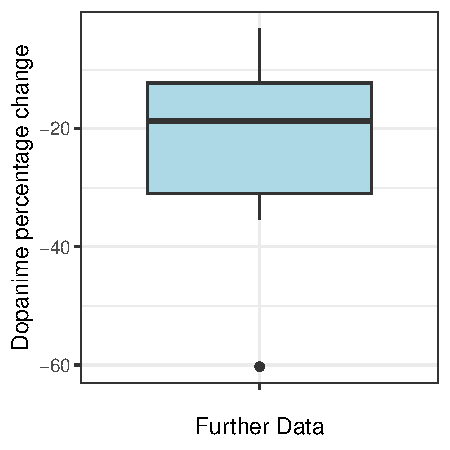
\includegraphics[width=\maxwidth]{figure/unnamed-chunk-5-1} 
\end{knitrout}
\caption{Boxplot showing percentage change in dopamine levels when zebra finches sing further away.}
\end{figure}
\begin{table}

\caption{\label{tab:unnamed-chunk-6}Numerical Summary of Dopamine Levels (Further Data)}
\centering
\begin{tabular}[t]{r|r|r|r|r|r|r}
\hline
mean & sd & min & q1 & median & q3 & max\\
\hline
-0.2027244 & 0.1303193 & -0.6027859 & -0.3092606 & -0.1867461 & -0.1227054 & -0.0299347\\
\hline
\end{tabular}
\end{table}


The data suggest that the dopamine in the brains of young zebra finches decreases when they sing further away. The numerical summary reflect the drop in the dopamine since all key measures of central tendency are negative. The maximum value is also negative. The entire boxplot lies below 0\% and there are no positive outliers.

\item Summarize the closer data. Do the data suggest that
   dopamine in the brains of young zebra finches increases when
   they sing closer to their adult song?
\begin{knitrout}\scriptsize
\definecolor{shadecolor}{rgb}{0.969, 0.969, 0.969}\color{fgcolor}\begin{kframe}
\begin{alltt}
\hldef{closer.dat} \hlkwb{<-} \hldef{fig.data}\hlopt{$}\hldef{closer_vals}

\hlcom{#do numerical summary for the data}
\hldef{closer.summary} \hlkwb{<-} \hlkwd{tibble}\hldef{(}
  \hlkwc{mean} \hldef{=} \hlkwd{mean}\hldef{(closer.dat),}
  \hlkwc{sd} \hldef{=} \hlkwd{sd}\hldef{(closer.dat),}
  \hlkwc{min} \hldef{=} \hlkwd{min}\hldef{(closer.dat),}
  \hlkwc{q1} \hldef{=} \hlkwd{quantile}\hldef{(closer.dat,} \hlkwc{probs} \hldef{=} \hlnum{0.25}\hldef{),}
  \hlkwc{median} \hldef{=} \hlkwd{quantile}\hldef{(closer.dat,} \hlkwc{probs} \hldef{=} \hlnum{0.50}\hldef{),}
  \hlkwc{q3} \hldef{=} \hlkwd{quantile}\hldef{(closer.dat,} \hlkwc{probs} \hldef{=} \hlnum{0.75}\hldef{),}
  \hlkwc{max} \hldef{=} \hlkwd{max}\hldef{(closer.dat)}
\hldef{)}

\hlcom{#do graphical summary for the data}
\hldef{closer.boxplot} \hlkwb{<-} \hlkwd{ggplot}\hldef{(}\hlkwc{data} \hldef{=} \hlkwd{tibble}\hldef{(closer.dat))}\hlopt{+}
  \hlkwd{geom_boxplot}\hldef{(}\hlkwd{aes}\hldef{(}\hlkwc{x} \hldef{=} \hlsng{""}\hldef{,} \hlkwc{y} \hldef{= closer.dat}\hlopt{*}\hlnum{100}\hldef{),}
            \hlkwc{fill} \hldef{=} \hlsng{"lightblue"}\hldef{)}\hlopt{+} \hlcom{#make the boxplot for the data}
  \hlkwd{theme_bw}\hldef{()}\hlopt{+}
  \hlkwd{xlab}\hldef{(}\hlsng{"Closer Data"}\hldef{)}\hlopt{+}
  \hlkwd{ylab}\hldef{(}\hlsng{"Dopanime percentage change"}\hldef{)}
\end{alltt}
\end{kframe}
\end{knitrout}

\begin{figure}[H]
\centering
\begin{knitrout}
\definecolor{shadecolor}{rgb}{0.969, 0.969, 0.969}\color{fgcolor}
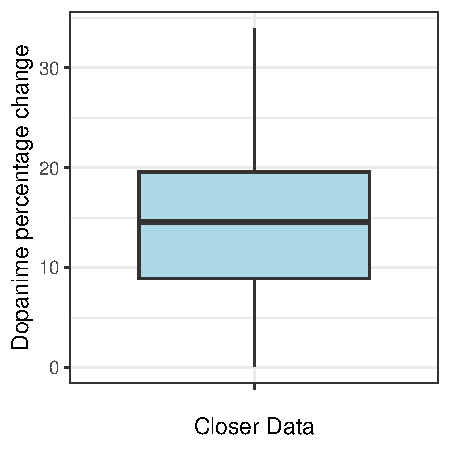
\includegraphics[width=\maxwidth]{figure/unnamed-chunk-8-1} 
\end{knitrout}
\caption{Boxplot showing percentage change in dopamine levels when zebra finches sing closer.}
\end{figure}
\begin{table}

\caption{\label{tab:unnamed-chunk-9}Numerical Summary of Dopamine Levels (Closer Data)}
\centering
\begin{tabular}[t]{r|r|r|r|r|r|r}
\hline
mean & sd & min & q1 & median & q3 & max\\
\hline
0.1562231 & 0.094083 & 0.0010821 & 0.089018 & 0.1455341 & 0.19567 & 0.3394881\\
\hline
\end{tabular}
\end{table}



The data suggest that dopamine in the brains of young zebra finches increases when they sing closer to their adult song. The values in numerical summaries are positive, indicating the increase in dopamine levels. The whole boxplot lies above 0, so the dopamine levels increases when zebra finches sing closer to their adult song.
  \item Summarize the paired differences. Do the data suggest
  that there is a difference between dopamine in the brains of
  young zebra finches when they sing further away compared to 
  closer to their adult song?
\begin{knitrout}\scriptsize
\definecolor{shadecolor}{rgb}{0.969, 0.969, 0.969}\color{fgcolor}\begin{kframe}
\begin{alltt}
\hldef{diff.dat} \hlkwb{<-} \hldef{fig.data}\hlopt{$}\hldef{difference}

\hlcom{#do numerical summary for the data}
\hldef{diff.summary} \hlkwb{<-} \hlkwd{tibble}\hldef{(}
\hlkwc{mean} \hldef{=} \hlkwd{mean}\hldef{(diff.dat),}
\hlkwc{sd} \hldef{=} \hlkwd{sd}\hldef{(diff.dat),}
\hlkwc{min} \hldef{=} \hlkwd{min}\hldef{(diff.dat),}
\hlkwc{q1} \hldef{=} \hlkwd{quantile}\hldef{(diff.dat,} \hlkwc{probs} \hldef{=} \hlnum{0.25}\hldef{),}
\hlkwc{median} \hldef{=} \hlkwd{quantile}\hldef{(diff.dat,} \hlkwc{probs} \hldef{=} \hlnum{0.50}\hldef{),}
\hlkwc{q3} \hldef{=} \hlkwd{quantile}\hldef{(diff.dat,} \hlkwc{probs} \hldef{=} \hlnum{0.75}\hldef{),}
\hlkwc{max} \hldef{=} \hlkwd{max}\hldef{(diff.dat)}
\hldef{)}

\hlcom{#do graphical summary for the data}
\hldef{diff.boxplot} \hlkwb{<-} \hlkwd{ggplot}\hldef{(}\hlkwc{data} \hldef{=} \hlkwd{tibble}\hldef{(diff.dat))}\hlopt{+}
\hlkwd{geom_boxplot}\hldef{(}\hlkwd{aes}\hldef{(}\hlkwc{x} \hldef{=} \hlsng{""}\hldef{,} \hlkwc{y} \hldef{= diff.dat}\hlopt{*}\hlnum{100}\hldef{),}
             \hlkwc{fill} \hldef{=} \hlsng{"lightblue"}\hldef{)}\hlopt{+} \hlcom{#make the boxplot for the data}
\hlkwd{theme_bw}\hldef{()}\hlopt{+}
\hlkwd{xlab}\hldef{(}\hlsng{"Paired difference"}\hldef{)}\hlopt{+}
\hlkwd{ylab}\hldef{(}\hlsng{"Dopanime percentage change"}\hldef{)}
\end{alltt}
\end{kframe}
\end{knitrout}

\begin{figure}[H]
\centering
\begin{knitrout}
\definecolor{shadecolor}{rgb}{0.969, 0.969, 0.969}\color{fgcolor}
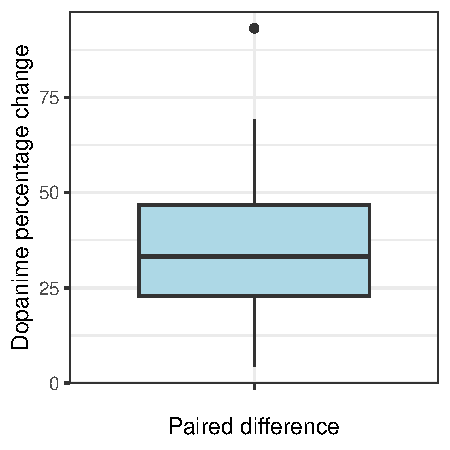
\includegraphics[width=\maxwidth]{figure/unnamed-chunk-11-1} 
\end{knitrout}
\caption{Boxplot showing percentage change in dopamine levels in paired difference of closer and further values.}
\end{figure}
\begin{table}

\caption{\label{tab:unnamed-chunk-12}Numerical Summary of Dopamine Levels (Paired Difference)}
\centering
\begin{tabular}[t]{r|r|r|r|r|r|r}
\hline
mean & sd & min & q1 & median & q3 & max\\
\hline
0.3589475 & 0.2108744 & 0.043353 & 0.2286407 & 0.3320846 & 0.4677148 & 0.9318804\\
\hline
\end{tabular}
\end{table}



The data suggest that there is a difference between dopamine in the brains of young zebra finches when they sing further away compared to closer to their adult song. The numerical summaries show that all paired differences are positive. This means that every bird had higher dopamine when it sang closer to its adult song compared to when it sang further away from its adult song. Also, the whole box plot lies above 0, which indicates dopamine increase for the closer conditions.
\end{enumerate}
%%%%%%%%%%%%%%%%%%%%%%%%%%%%%%%%%%%%%%%%%%%%%%%%%%%%%%%%%%%%%%%%%
% CONDUCT THE TESTS
%%%%%%%%%%%%%%%%%%%%%%%%%%%%%%%%%%%%%%%%%%%%%%%%%%%%%%%%%%%%%%%%%
\item Conduct the inferences they do in the paper. Make sure to report the results
a little more comprehensively -- that is your parenthetical should look something
like: ($t=23.99$, $p<0.0001$; $g=1.34$; 95\% CI: 4.43, 4.60).\\
\textbf{Note:} Your numbers may vary slightly as they performed some unclear
correction of their $p$-values. I'm waiting to hear back from them via email!
\begin{enumerate}
  \item ``The close responses differed significantly from 0 ($p=1.63 \times 10^{-8}$).''
\begin{knitrout}\scriptsize
\definecolor{shadecolor}{rgb}{0.969, 0.969, 0.969}\color{fgcolor}\begin{kframe}
\begin{alltt}
\hldef{conf.level} \hlkwb{=} \hlnum{0.95}
\hldef{mu0} \hlkwb{<-} \hlnum{0}
\hlcom{#part a - conduct t-test for close responses}
\hldef{p.val.close} \hlkwb{<-} \hlkwd{t.test}\hldef{(}\hlkwc{x}\hldef{=closer.dat,} \hlkwc{mu} \hldef{= mu0,} \hlkwc{alternative} \hldef{=} \hlsng{"greater"}\hldef{)}
\hlcom{#get values for parenthesis}
\hldef{conf.int.close} \hlkwb{<-} \hldef{p.val.close}\hlopt{$}\hldef{conf.int} \hlcom{#get the confidence interval}
\hldef{conf.close.beg} \hlkwb{<-} \hldef{conf.int.close[}\hlnum{1}\hldef{]}
\hldef{conf.close.end} \hlkwb{<-} \hldef{conf.int.close[}\hlnum{2}\hldef{]}
\hldef{t.close} \hlkwb{<-} \hldef{p.val.close}\hlopt{$}\hldef{statistic} \hlcom{#get t}
\hldef{df.close} \hlkwb{<-} \hldef{p.val.close}\hlopt{$}\hldef{parameter} \hlcom{#get df}
\hldef{g.close} \hlkwb{<-} \hlkwd{hedges_g}\hldef{(}\hlkwc{x} \hldef{= closer.dat,} \hlkwc{mu} \hldef{= mu0,} \hlkwc{alternative} \hldef{=} \hlsng{"greater"}\hldef{)} \hlcom{#get g}
\hldef{n.close} \hlkwb{<-} \hldef{p.val.close}\hlopt{$}\hldef{parameter} \hlopt{+} \hlnum{1}
\hldef{s.close} \hlkwb{<-} \hldef{p.val.close}\hlopt{$}\hldef{stderr} \hlopt{*} \hlkwd{sqrt}\hldef{(n.close)}
\hlcom{#get p-value}
\hldef{p.val.close} \hlkwb{<-} \hldef{p.val.close}\hlopt{$}\hldef{p.value}
\end{alltt}
\end{kframe}
\end{knitrout}

The close responses are statistically discernible from 0 ($t=8.3$, $p< 0.0001$; $g=1.61$; one-sided 95\% CI: 0.12, \ensuremath{\infty{}}).
  \item ``The far responses differed significantly from 0 ($p=5.17 \times 10^{-8}$).''
\begin{knitrout}\scriptsize
\definecolor{shadecolor}{rgb}{0.969, 0.969, 0.969}\color{fgcolor}\begin{kframe}
\begin{alltt}
\hldef{p.val.far} \hlkwb{<-} \hlkwd{t.test}\hldef{(}\hlkwc{x}\hldef{=further.dat,} \hlkwc{mu} \hldef{= mu0,} \hlkwc{alternative} \hldef{=} \hlsng{"less"}\hldef{)}
\hlcom{#get values for parenthesis}
\hldef{conf.int.far} \hlkwb{<-} \hldef{p.val.far}\hlopt{$}\hldef{conf.int} \hlcom{#get the confidence interval}
\hldef{conf.far.beg} \hlkwb{<-} \hldef{conf.int.far[}\hlnum{1}\hldef{]}
\hldef{conf.far.end} \hlkwb{<-} \hldef{conf.int.far[}\hlnum{2}\hldef{]}
\hldef{t.far} \hlkwb{<-} \hldef{p.val.far}\hlopt{$}\hldef{statistic} \hlcom{#get t }
\hldef{df.far} \hlkwb{<-} \hldef{p.val.far}\hlopt{$}\hldef{parameter} \hlcom{#get df}
\hldef{g.far} \hlkwb{<-} \hlkwd{hedges_g}\hldef{(}\hlkwc{x} \hldef{= further.dat,} \hlkwc{mu} \hldef{= mu0,} \hlkwc{alternative} \hldef{=} \hlsng{"less"}\hldef{)} \hlcom{#get g}
\hldef{n.far} \hlkwb{<-} \hldef{p.val.far}\hlopt{$}\hldef{parameter} \hlopt{+} \hlnum{1}
\hldef{s.far} \hlkwb{<-} \hldef{p.val.far}\hlopt{$}\hldef{stderr} \hlopt{*} \hlkwd{sqrt}\hldef{(n.far)}
\hlcom{#get p-value}
\hldef{p.val.far} \hlkwb{<-} \hldef{p.val.far}\hlopt{$}\hldef{p.value}
\end{alltt}
\end{kframe}
\end{knitrout}
The far responses are statistically discernible from 0 ($t=-7.78$, $p< 0.0001$; $g=-1.51$; one-sided 95\% CI: \ensuremath{-\infty{}}, -0.16).
  \item ``The difference between populations was significant ($p=1.04 \times10^{-8}$).''
\begin{knitrout}\scriptsize
\definecolor{shadecolor}{rgb}{0.969, 0.969, 0.969}\color{fgcolor}\begin{kframe}
\begin{alltt}
\hldef{p.val.diff} \hlkwb{<-} \hlkwd{t.test}\hldef{(}\hlkwc{x}\hldef{=diff.dat,} \hlkwc{mu} \hldef{= mu0,} \hlkwc{alternative} \hldef{=} \hlsng{"two.sided"}\hldef{)}
\hlcom{#get values for parenthesis}
\hldef{conf.int.diff} \hlkwb{<-} \hldef{p.val.diff}\hlopt{$}\hldef{conf.int} \hlcom{#get the confidence interval}
\hldef{conf.diff.beg} \hlkwb{<-} \hldef{conf.int.diff[}\hlnum{1}\hldef{]}
\hldef{conf.diff.end} \hlkwb{<-} \hldef{conf.int.diff[}\hlnum{2}\hldef{]}
\hldef{t.diff} \hlkwb{<-} \hldef{p.val.diff}\hlopt{$}\hldef{statistic} \hlcom{#get t }
\hldef{df.diff} \hlkwb{<-} \hldef{p.val.diff}\hlopt{$}\hldef{parameter} \hlcom{#get df}
\hldef{g.diff} \hlkwb{<-} \hlkwd{hedges_g}\hldef{(}\hlkwc{x} \hldef{= diff.dat,} \hlkwc{mu} \hldef{= mu0,} \hlkwc{alternative} \hldef{=} \hlsng{"two.sided"}\hldef{)} \hlcom{#get g}
\hldef{n.diff} \hlkwb{<-} \hldef{p.val.diff}\hlopt{$}\hldef{parameter} \hlopt{+} \hlnum{1}
\hldef{s.diff} \hlkwb{<-} \hldef{p.val.diff}\hlopt{$}\hldef{stderr} \hlopt{*} \hlkwd{sqrt}\hldef{(n.diff)}
\hlcom{#get p-value}
\hldef{p.val.diff} \hlkwb{<-} \hldef{p.val.diff}\hlopt{$}\hldef{p.value}
\end{alltt}
\end{kframe}
\end{knitrout}
The difference between populations are statistically discernible ($t=8.51$, $p< 0.0001$; $g=1.65$; two-sided 95\% CI: 0.27, 0.45).
\end{enumerate}
%%%%%%%%%%%%%%%%%%%%%%%%%%%%%%%%%%%%%%%%%%%%%%%%%%%%%%%%%%%%%%%%%
% CONDUCT THE TESTS
%%%%%%%%%%%%%%%%%%%%%%%%%%%%%%%%%%%%%%%%%%%%%%%%%%%%%%%%%%%%%%%%%
\item Reverse engineer the hypothesis test plot from Lecture 20 to create accurate
hypothesis testing plots for each part of the previous question.
\begin{enumerate}
  \item Question 4, part(a).
\begin{knitrout}\scriptsize
\definecolor{shadecolor}{rgb}{0.969, 0.969, 0.969}\color{fgcolor}\begin{kframe}
\begin{alltt}
\hlcom{# For plotting the null distribution}
\hldef{ggdat.t.close} \hlkwb{<-} \hlkwd{tibble}\hldef{(}\hlkwc{t}\hldef{=}\hlkwd{seq}\hldef{(}\hlopt{-}\hlnum{10}\hldef{,}\hlnum{10}\hldef{,}\hlkwc{length.out}\hldef{=}\hlnum{1000}\hldef{))|>}
\hlkwd{mutate}\hldef{(}\hlkwc{pdf.null} \hldef{=} \hlkwd{dt}\hldef{(}\hlkwc{x}\hldef{=t,} \hlkwc{df}\hldef{=df.close))}
\hlcom{# For plotting the observed point}
\hldef{ggdat.obs.close} \hlkwb{<-} \hlkwd{tibble}\hldef{(}\hlkwc{t} \hldef{= t.close,}
                        \hlkwc{y} \hldef{=} \hlnum{0}\hldef{)} \hlcom{# to plot on x-axis}
\hldef{t.breaks} \hlkwb{<-} \hlkwd{c}\hldef{(}\hlopt{-}\hlnum{5}\hldef{,} \hlkwd{qt}\hldef{(}\hlkwc{p} \hldef{=} \hlnum{1}\hlopt{-}\hlnum{0.05}\hldef{,} \hlkwc{df} \hldef{= df.close),} \hlcom{# rejection region (left)}
            \hlnum{0}\hldef{,} \hlnum{5}\hldef{, t.close)}                  \hlcom{# t-statistic observed}
\hldef{t.breaks} \hlkwb{<-} \hlkwd{sort}\hldef{(}\hlkwd{unique}\hldef{(}\hlkwd{round}\hldef{(t.breaks,} \hlnum{2}\hldef{)))}
\hldef{xbar.breaks} \hlkwb{<-} \hldef{t.breaks} \hlopt{*} \hldef{s.close}\hlopt{/}\hlkwd{sqrt}\hldef{(n.close)} \hlopt{+} \hldef{mu0}
\hlcom{#plot for part a - close responses}
\hldef{close.plot} \hlkwb{<-} \hlkwd{ggplot}\hldef{()} \hlopt{+}
\hlcom{# null distribution}
\hlkwd{geom_line}\hldef{(}\hlkwc{data}\hldef{=ggdat.t.close,}
          \hlkwd{aes}\hldef{(}\hlkwc{x}\hldef{=t,} \hlkwc{y}\hldef{=pdf.null),} \hlkwc{color} \hldef{=} \hlsng{"black"}\hldef{)}\hlopt{+}
\hlkwd{geom_hline}\hldef{(}\hlkwc{yintercept}\hldef{=}\hlnum{0}\hldef{)}\hlopt{+}
\hlcom{# rejection regions}
\hlkwd{geom_ribbon}\hldef{(}\hlkwc{data}\hldef{=}\hlkwd{subset}\hldef{(ggdat.t.close, t}\hlopt{>=}\hlkwd{qt}\hldef{(}\hlkwc{p} \hldef{=} \hlnum{1}\hlopt{-}\hlnum{0.05}\hldef{,} \hlkwc{df}\hldef{=df.close)),}
            \hlkwd{aes}\hldef{(}\hlkwc{x}\hldef{=t,} \hlkwc{ymin}\hldef{=}\hlnum{0}\hldef{,} \hlkwc{ymax}\hldef{=pdf.null),}
            \hlkwc{fill}\hldef{=}\hlsng{"gray"}\hldef{,} \hlkwc{alpha}\hldef{=}\hlnum{0.5}\hldef{)}\hlopt{+}
\hlcom{# plot p-value (not visible)}
\hlkwd{geom_ribbon}\hldef{(}\hlkwc{data}\hldef{=}\hlkwd{subset}\hldef{(ggdat.t.close, t}\hlopt{>=}\hldef{t.close),}
            \hlkwd{aes}\hldef{(}\hlkwc{x}\hldef{=t,} \hlkwc{ymin}\hldef{=}\hlnum{0}\hldef{,} \hlkwc{ymax}\hldef{=pdf.null),}
            \hlkwc{fill}\hldef{=}\hlsng{"red"}\hldef{,} \hlkwc{alpha}\hldef{=}\hlnum{0.25}\hldef{)}\hlopt{+}
\hlcom{# plot observation point}
\hlkwd{geom_point}\hldef{(}\hlkwc{data}\hldef{=ggdat.obs.close,} \hlkwd{aes}\hldef{(}\hlkwc{x}\hldef{=t,} \hlkwc{y}\hldef{=y),} \hlkwc{color}\hldef{=}\hlsng{"red"}\hldef{)}\hlopt{+}
\hlkwd{theme_bw}\hldef{()}\hlopt{+}
\hlkwd{ylab}\hldef{(}\hlsng{"Density"}\hldef{)}\hlopt{+}
\hlkwd{scale_x_continuous}\hldef{(}\hlsng{"t"}\hldef{,}
                   \hlkwc{breaks} \hldef{=} \hlkwd{round}\hldef{(t.breaks,}\hlnum{2}\hldef{),}
                   \hlkwc{sec.axis} \hldef{=} \hlkwd{sec_axis}\hldef{(}\hlopt{~}\hldef{.,}
                                       \hlkwc{name} \hldef{=} \hlkwd{bquote}\hldef{(}\hlkwd{bar}\hldef{(x)),}
                                       \hlkwc{breaks} \hldef{= t.breaks,}
                                       \hlkwc{labels} \hldef{=} \hlkwd{round}\hldef{(xbar.breaks,}\hlnum{2}\hldef{)))}\hlopt{+}
\hlkwd{ggtitle}\hldef{(}\hlsng{"T-Test for Mean Dopamine Level of Close Responses"}\hldef{,}
        \hlkwc{subtitle}\hldef{=}\hlkwd{bquote}\hldef{(H[}\hlnum{0}\hldef{]}\hlopt{==}\hlnum{0}\hlopt{*}\hlsng{";"}\hlopt{~}\hldef{H[a]}\hlopt{>}\hlnum{0}\hldef{))}
\end{alltt}
\end{kframe}
\end{knitrout}
\begin{figure}[H]
\centering
\begin{knitrout}
\definecolor{shadecolor}{rgb}{0.969, 0.969, 0.969}\color{fgcolor}
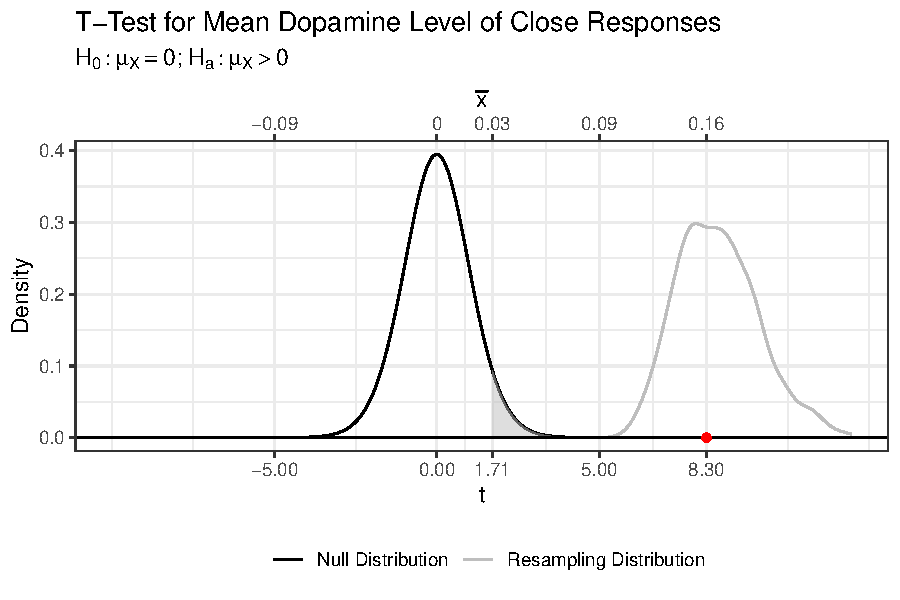
\includegraphics[width=\maxwidth]{figure/unnamed-chunk-17-1} 
\end{knitrout}
\caption{T-Test for Mean Dopamine Level of Difference in Close Responses for Zebra Finches.}
\end{figure}
  \item Question 4, part(b).
\begin{knitrout}\scriptsize
\definecolor{shadecolor}{rgb}{0.969, 0.969, 0.969}\color{fgcolor}\begin{kframe}
\begin{alltt}
\hlcom{# For plotting the null distribution}
\hldef{ggdat.t.far} \hlkwb{<-} \hlkwd{tibble}\hldef{(}\hlkwc{t}\hldef{=}\hlkwd{seq}\hldef{(}\hlopt{-}\hlnum{10}\hldef{,}\hlnum{10}\hldef{,}\hlkwc{length.out}\hldef{=}\hlnum{1000}\hldef{))|>}
\hlkwd{mutate}\hldef{(}\hlkwc{pdf.null} \hldef{=} \hlkwd{dt}\hldef{(}\hlkwc{x}\hldef{=t,} \hlkwc{df}\hldef{=df.far))}
\hlcom{# For plotting the observed point}
\hldef{ggdat.obs.far} \hlkwb{<-} \hlkwd{tibble}\hldef{(}\hlkwc{t} \hldef{= t.far,}
                        \hlkwc{y} \hldef{=} \hlnum{0}\hldef{)} \hlcom{# to plot on x-axis}
\hldef{t.breaks} \hlkwb{<-} \hlkwd{c}\hldef{(}\hlopt{-}\hlnum{5}\hldef{,} \hlkwd{qt}\hldef{(}\hlkwc{p} \hldef{=} \hlnum{0.05}\hldef{,} \hlkwc{df} \hldef{= df.far),} \hlcom{# rejection region (left)}
            \hlnum{0}\hldef{,} \hlnum{5}\hldef{, t.far)}                  \hlcom{# t-statistic observed}
\hldef{t.breaks} \hlkwb{<-} \hlkwd{sort}\hldef{(}\hlkwd{unique}\hldef{(}\hlkwd{round}\hldef{(t.breaks,} \hlnum{2}\hldef{)))}
\hldef{xbar.breaks} \hlkwb{<-} \hldef{t.breaks} \hlopt{*} \hldef{s.far}\hlopt{/}\hlkwd{sqrt}\hldef{(n.far)} \hlopt{+} \hldef{mu0}
\hlcom{#plot for part a - far responses}
\hldef{far.plot} \hlkwb{<-} \hlkwd{ggplot}\hldef{()} \hlopt{+}
\hlcom{# null distribution}
\hlkwd{geom_line}\hldef{(}\hlkwc{data}\hldef{=ggdat.t.far,}
          \hlkwd{aes}\hldef{(}\hlkwc{x}\hldef{=t,} \hlkwc{y}\hldef{=pdf.null),} \hlkwc{color} \hldef{=} \hlsng{"black"}\hldef{)}\hlopt{+}
\hlkwd{geom_hline}\hldef{(}\hlkwc{yintercept}\hldef{=}\hlnum{0}\hldef{)}\hlopt{+}
\hlcom{# rejection regions}
\hlkwd{geom_ribbon}\hldef{(}\hlkwc{data}\hldef{=}\hlkwd{subset}\hldef{(ggdat.t.far, t}\hlopt{<=}\hlkwd{qt}\hldef{(}\hlkwc{p} \hldef{=} \hlnum{0.05}\hldef{,} \hlkwc{df}\hldef{=df.far)),}
            \hlkwd{aes}\hldef{(}\hlkwc{x}\hldef{=t,} \hlkwc{ymin}\hldef{=}\hlnum{0}\hldef{,} \hlkwc{ymax}\hldef{=pdf.null),}
            \hlkwc{fill}\hldef{=}\hlsng{"gray"}\hldef{,} \hlkwc{alpha}\hldef{=}\hlnum{0.5}\hldef{)}\hlopt{+}
\hlcom{# plot observation point}
\hlkwd{geom_point}\hldef{(}\hlkwc{data}\hldef{=ggdat.obs.far,} \hlkwd{aes}\hldef{(}\hlkwc{x}\hldef{=t,} \hlkwc{y}\hldef{=y),} \hlkwc{color}\hldef{=}\hlsng{"red"}\hldef{)}\hlopt{+}
\hlkwd{theme_bw}\hldef{()}\hlopt{+}
\hlkwd{ylab}\hldef{(}\hlsng{"Density"}\hldef{)}\hlopt{+}
\hlkwd{scale_x_continuous}\hldef{(}\hlsng{"t"}\hldef{,}
                   \hlkwc{breaks} \hldef{=} \hlkwd{round}\hldef{(t.breaks,}\hlnum{2}\hldef{),}
                   \hlkwc{sec.axis} \hldef{=} \hlkwd{sec_axis}\hldef{(}\hlopt{~}\hldef{.,}
                                       \hlkwc{name} \hldef{=} \hlkwd{bquote}\hldef{(}\hlkwd{bar}\hldef{(x)),}
                                       \hlkwc{breaks} \hldef{= t.breaks,}
                                       \hlkwc{labels} \hldef{=} \hlkwd{round}\hldef{(xbar.breaks,}\hlnum{2}\hldef{)))}\hlopt{+}
\hlkwd{ggtitle}\hldef{(}\hlsng{"T-Test for Mean Dopamine Level of Far Responses for Zebra Finches "}\hldef{,}
        \hlkwc{subtitle}\hldef{=}\hlkwd{bquote}\hldef{(H[}\hlnum{0}\hldef{]}\hlopt{==}\hlnum{0}\hlopt{*}\hlsng{";"}\hlopt{~}\hldef{H[a]}\hlopt{<}\hlnum{0}\hldef{))}
\end{alltt}
\end{kframe}
\end{knitrout}
\begin{figure}[H]
\centering
\begin{knitrout}
\definecolor{shadecolor}{rgb}{0.969, 0.969, 0.969}\color{fgcolor}
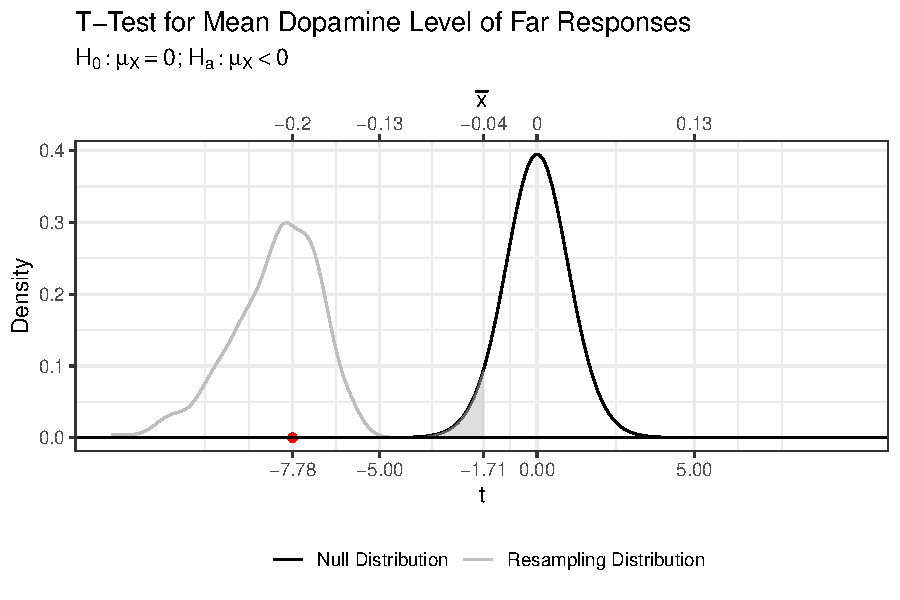
\includegraphics[width=\maxwidth]{figure/unnamed-chunk-19-1} 
\end{knitrout}
\caption{T-Test for Mean Dopamine Level of Far Responses for Zebra Finches.}
\end{figure}
  \item Question 4, part(c).
\begin{knitrout}\scriptsize
\definecolor{shadecolor}{rgb}{0.969, 0.969, 0.969}\color{fgcolor}\begin{kframe}
\begin{alltt}
\hlcom{# For plotting the null distribution}
\hldef{ggdat.t.diff} \hlkwb{<-} \hlkwd{tibble}\hldef{(}\hlkwc{t}\hldef{=}\hlkwd{seq}\hldef{(}\hlopt{-}\hlnum{10}\hldef{,}\hlnum{10}\hldef{,}\hlkwc{length.out}\hldef{=}\hlnum{1000}\hldef{))|>}
\hlkwd{mutate}\hldef{(}\hlkwc{pdf.null} \hldef{=} \hlkwd{dt}\hldef{(}\hlkwc{x}\hldef{=t,} \hlkwc{df}\hldef{=df.diff))}
\hlcom{# For plotting the observed point}
\hldef{ggdat.obs.diff} \hlkwb{<-} \hlkwd{tibble}\hldef{(}\hlkwc{t} \hldef{= t.diff,}
                      \hlkwc{y} \hldef{=} \hlnum{0}\hldef{)} \hlcom{# to plot on x-axis}
\hldef{t.breaks} \hlkwb{<-} \hlkwd{c}\hldef{(}\hlopt{-}\hlnum{5}\hldef{,} \hlkwd{qt}\hldef{(}\hlkwc{p} \hldef{=} \hlnum{0.025}\hldef{,} \hlkwc{df} \hldef{= df.diff),} \hlcom{# rejection region (left)}
            \hlnum{0}\hldef{,} \hlkwd{qt}\hldef{(}\hlkwc{p} \hldef{=} \hlnum{1}\hlopt{-}\hlnum{0.025}\hldef{,} \hlkwc{df} \hldef{= df.diff),} \hlnum{5}\hldef{, t.diff)}                  \hlcom{# t-statistic observed}
\hldef{t.breaks} \hlkwb{<-} \hlkwd{sort}\hldef{(}\hlkwd{unique}\hldef{(}\hlkwd{round}\hldef{(t.breaks,} \hlnum{2}\hldef{)))}
\hldef{xbar.breaks} \hlkwb{<-} \hldef{t.breaks} \hlopt{*} \hldef{s.diff}\hlopt{/}\hlkwd{sqrt}\hldef{(n.diff)} \hlopt{+} \hldef{mu0}
\hlcom{#plot for part a - diff responses}
\hldef{diff.plot} \hlkwb{<-} \hlkwd{ggplot}\hldef{()} \hlopt{+}
\hlcom{# null distribution}
\hlkwd{geom_line}\hldef{(}\hlkwc{data}\hldef{=ggdat.t.diff,}
          \hlkwd{aes}\hldef{(}\hlkwc{x}\hldef{=t,} \hlkwc{y}\hldef{=pdf.null),} \hlkwc{color} \hldef{=} \hlsng{"black"}\hldef{)}\hlopt{+}
\hlkwd{geom_hline}\hldef{(}\hlkwc{yintercept}\hldef{=}\hlnum{0}\hldef{)}\hlopt{+}
\hlcom{# rejection regions}
\hlkwd{geom_ribbon}\hldef{(}\hlkwc{data}\hldef{=}\hlkwd{subset}\hldef{(ggdat.t.diff, t}\hlopt{<=}\hlkwd{qt}\hldef{(}\hlkwc{p} \hldef{=} \hlnum{0.025}\hldef{,} \hlkwc{df}\hldef{=df.diff)),}
            \hlkwd{aes}\hldef{(}\hlkwc{x}\hldef{=t,} \hlkwc{ymin}\hldef{=}\hlnum{0}\hldef{,} \hlkwc{ymax}\hldef{=pdf.null),}
            \hlkwc{fill}\hldef{=}\hlsng{"gray"}\hldef{,} \hlkwc{alpha}\hldef{=}\hlnum{0.5}\hldef{)}\hlopt{+}
\hlkwd{geom_ribbon}\hldef{(}\hlkwc{data}\hldef{=}\hlkwd{subset}\hldef{(ggdat.t.diff, t}\hlopt{>=}\hlkwd{qt}\hldef{(}\hlnum{0.975}\hldef{,} \hlkwc{df}\hldef{=df.diff)),}
            \hlkwd{aes}\hldef{(}\hlkwc{x}\hldef{=t,} \hlkwc{ymin}\hldef{=}\hlnum{0}\hldef{,} \hlkwc{ymax}\hldef{=pdf.null),}
            \hlkwc{fill}\hldef{=}\hlsng{"grey"}\hldef{,} \hlkwc{alpha}\hldef{=}\hlnum{0.5}\hldef{)}\hlopt{+}
\hlcom{# plot observation point}
\hlkwd{geom_point}\hldef{(}\hlkwc{data}\hldef{=ggdat.obs.diff,} \hlkwd{aes}\hldef{(}\hlkwc{x}\hldef{=t,} \hlkwc{y}\hldef{=y),} \hlkwc{color}\hldef{=}\hlsng{"red"}\hldef{)}\hlopt{+}
\hlkwd{theme_bw}\hldef{()}\hlopt{+}
\hlkwd{ylab}\hldef{(}\hlsng{"Density"}\hldef{)}\hlopt{+}
\hlkwd{scale_x_continuous}\hldef{(}\hlsng{"t"}\hldef{,}
                   \hlkwc{breaks} \hldef{=} \hlkwd{round}\hldef{(t.breaks,}\hlnum{2}\hldef{),}
                   \hlkwc{sec.axis} \hldef{=} \hlkwd{sec_axis}\hldef{(}\hlopt{~}\hldef{.,}
                                       \hlkwc{name} \hldef{=} \hlkwd{bquote}\hldef{(}\hlkwd{bar}\hldef{(x)),}
                                       \hlkwc{breaks} \hldef{= t.breaks,}
                                       \hlkwc{labels} \hldef{=} \hlkwd{round}\hldef{(xbar.breaks,}\hlnum{2}\hldef{)))}\hlopt{+}
\hlkwd{ggtitle}\hldef{(}\hlsng{"T-Test for Mean Dopamine Level of Difference in Responses"}\hldef{,}
        \hlkwc{subtitle}\hldef{=}\hlkwd{bquote}\hldef{(H[}\hlnum{0}\hldef{]}\hlopt{==}\hlnum{0}\hlopt{*}\hlsng{";"}\hlopt{~}\hldef{H[a]} \hlopt{!=} \hlnum{0}\hldef{))}
\end{alltt}
\end{kframe}
\end{knitrout}
\begin{figure}[H]
\centering
\begin{knitrout}
\definecolor{shadecolor}{rgb}{0.969, 0.969, 0.969}\color{fgcolor}
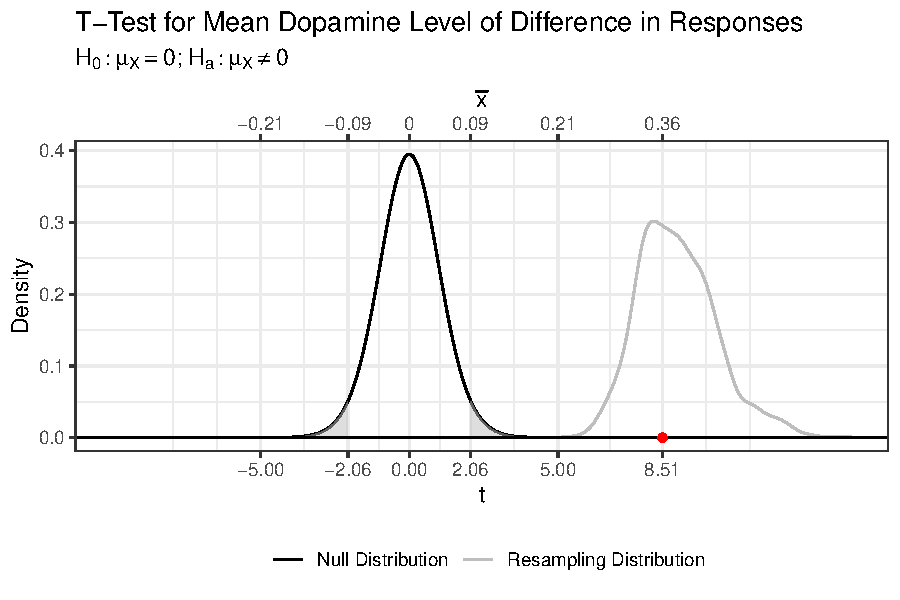
\includegraphics[width=\maxwidth]{figure/unnamed-chunk-21-1} 
\end{knitrout}
\caption{T-Test for Mean Dopamine Level of Difference in Responses for Zebra Finches.}
\end{figure}
\end{enumerate}
\end{enumerate}


\bibliography{bibliography}
\end{document}
